\chapter{Background}\label{chap:background}

This chapter covers the background on the range of different topics which are important to this thesis. It starts by explaining transactional memory~(Section~\ref{chap:TM}) and sharing-aware mapping~(Section~\ref{sect:sharing-aware}). Benchmarks for STM are briefly described in Section~\ref{sec:STAMP}. We also include a small experiment to show the benefits of sharing-aware thread mapping for STM applications~(Section~\ref{sec:improvements}).

\section{Transactional Memory}\label{chap:TM}

Transactional memory (TM) is an abstraction to synchronize accesses to shared variables. Instead of using locks, the programmer only needs to enclose the critical section in an atomic block, which will be executed as a transaction. The concept of transactions was borrowed from Databases. In fact, the first idea to use Database transactions in programming languages was described by \citeNamesYearPar{Lomet:1977}. Sixteen years later, \citeNamesYearPar{Herlihy:1993} proposed hardware support for TM. The first implementation purely on software (STM) was proposed by \citeNamesYearPar{Shavit:1995} as a flexible alternative not dependent on hardware. There are also hybrid approaches \cite{Damron:2006} that combine implementation both on hardware and software.


\subsection{General Concepts}\label{sec:TMConcepts}

The execution of a transaction needs to be \emph{atomic}. Atomicity requires that a transaction is executed as a whole or it needs to appear as it was never executed \cite{Harris:2010, Grahn:2010}. This property is also known as ``all-or-nothing'' \cite{Ozsu:1996}. A transaction \emph{commits} if executed without conflicts, hence all operations and results are made visible to the rest of the system \cite{Grahn:2010}. If conflicts are detected, a transaction \emph{aborts}, i.e., all operations are discarded, and the transaction needs to restart until a commit is possible. This idea is associated with another important property called \emph{isolation}: all memory updates of a running transaction can not be visible to other transactions before a commit.

The sequence of operations performed by all transactions in a given execution is called \emph{history} \cite{Opacity}. If one transaction executes only after the end of the other they are serial, otherwise \emph{concurrent} \cite{Harris:2010}. If they are concurrent, conflicts could occur between them. A conflict occurs when two transactions perform operations in the same memory location, and at least one of these operations is a write. 

As transactions can execute concurrently, correctness criteria were proposed to ensure that the TM system produces correct results. One of the most used criteria is \emph{Opacity} \cite{Opacity}, that is an extension of the classical database criteria \emph{Strict Serializability} \cite{Papadimitriou:1979}. Serializability says that the result of executing concurrent transactions in a given history must be equal to a serial execution. \emph{Strict Serializability} says that real-time order must be respected. If $T_1$ finishes before $T_2$ starts, then $T_1$ must occur before $T_2$ in the equivalent serial execution \cite{Harris:2010}. Opacity extends these concepts to aborted transactions, i.e., all transactions in a given history, including aborted, must appear to be executed in a serial order. %There are weaker alternatives proposed after Opacity, for instance, \emph{Virtual World} \cite{VWCFull} and \emph{Stricter Serializability} (SSER+) \cite{Sutra:2018}. 

%%%%%%%%%%%%%%%%%%%%%%%%%%%%%%%%%%%%%%%%%%%%%%%%%%%%%%%%%%%%%%%%%%%%
\subsection{Design Choices}\label{sec:TMDesignChoices}

Although the main purpose of TM is to provide a simple interface to manage accesses to shared resources, its implementation is not trivial. Many different design options are available such as transaction granularity, version management, conflict detection and resolution. The next subsections describe these design options.

\subsubsection{Version Management}\label{sec:versionManag}

TMs use version management of memory locations to manage the writes of concurrent transactions. Two approaches are used \cite{Harris:2010, TinySTM2}:

\begin{itemize}
	\item \textbf{Eager}, \textbf{direct update} or \textbf{write-through}: data is modified directly in memory. Older values are stored in an \emph{undo-log}. In case of an abort the log is used to restore the old values.
	
	\item \textbf{Lazy}, \textbf{deferred update} or \textbf{write-back}: instead of updating data directly in memory, new values are stored in an \emph{redo-log}. During a commit, the log is used to set new values to memory.  In case of an abort, the log is discarded.
\end{itemize}

Eager versioning makes committing faster, whereas lazy versioning makes aborting faster \cite{Grahn:2010}.

\subsubsection{Transaction Granularity}\label{sec:granularity}

The granularity is the dimension used for conflict detection, i.e., the level used for keeping track of memory locations. One option is to use memory \textbf{word} granularity. The main advantage is that no false conflicts happen. However it adds a high overhead in terms of time and space to keep the metadata \cite{Grahn:2010}. \textbf{Object} granularity is most used in object-based languages \cite{CastroPhD:2012}. However it can lead to false conflicts, i.e., transactions accessing the same object but different fields \cite{Larus:2008}. For HTM, \textbf{cache line} granularity is the most suitable~\cite{Grahn:2010}.

\subsubsection{Conflict Detection}\label{sec:conflictDetection}
Similar to version management, there are two approaches to deal with conflict detection between concurrent transactions \cite{Grahn:2010}:

\begin{itemize}
	\item \textbf{Eager}, \textbf{early}, \textbf{pessimistic} or \textbf{encounter-time}: conflicts are verified on each memory location read or written exactly when it occurs. In STM this could be done using locks or version number on memory locations. Thus, to access a value, a transaction needs to acquire its ownership, preventing others from accessing it \cite{Bandeira:2015}.
	
	\item \textbf{Lazy}, \textbf{late}, \textbf{optimistic} or \textbf{commit-time}: conflicts are verified only at commit time. It allows multiple transactions to access shared data and continue executing even if they conflict, as the TM system will detect and resolve them on commit time~\cite[p. 20]{Harris:2010}.
	
	%A transaction must validate all its read set in order to verify if any conflict with other transactions occurred. 
\end{itemize}

These options could be combined, for instance, lazy conflict detection for reads and eager for writes \cite{Bandeira:2015}.

\subsubsection{Conflict Resolution}\label{sec:contetionManager}

All operations executed by a transaction that aborts could be seen as a wasted work \cite{Spear:2009, Ansari:2009:PTM, Zhou:2016}. Thus, the total aborts in an execution have a strong relationship with the final performance. In case of conflicts, choosing which transaction needs to be aborted is a responsibility of the \emph{Contention Manager} (CM) \cite{Yoo:2008}. When two transactions $T_A$ and $T_B$ conflict, the transaction that has detected the conflict, suppose $T_A$, asks  the CM what to do. The actions could be, for instance, abort immediately or wait a determined time, allowing $T_B$ to finish, or force and abort of $T_B$~\cite{Guerraoui:2006}. 
There are many CMs proposed in the literature with different purposes. A few examples of them are \cite{Scherer:2005, Spear:2009, Harris:2010, Grahn:2010}: 
\begin{itemize}
	\item \textbf{Passive}: the transaction that detected the conflict aborts and restart its execution.
	
	\item \textbf{Polite}: the transaction that detected the conflict could abort the conflicting one. However,  aborting is delayed for a period of time, waiting the conflicting transaction to end accessing values. The transaction can also wait for a fixed number of exponentially growing intervals
	before aborting the enemy.
	
	\item \textbf{Karma}: use priorities to define which transaction must abort. The priority is defined by the total of memory locations that a transaction has accessed. The total is cumulative, i.e., taking in consideration all aborts and re-executions.
	
	\item \textbf{Timestamp}: aborts the transaction that started earlier.
	
	\item \textbf{Polka}: a hybrid between \textit{Polite} and \textit{Karma}.
	%As demonstrated in \cite{Scherer:2005}, the CM that achieved best performance were \textit{Polite} and \textit{Karma}. Thus, \textit{Polka} is a hybrid between the two.
\end{itemize}

%%%%%%%%%%%%%%%%%%%%%%%%%%%%%%%%%%%%%%%%%%%%%%%%%%%%%%%%%%%%%%%%%%%%
\subsection{STM Implementation}\label{sec:implementationTM}

The first STM implementations were non-blocking \cite{Shavit:1997}, more specifically obstruction-free \cite{Herlihy:2003_2}. However, according to \citeNamesYearPar{Ennals:2006}, obstruction-free is essential in distributed systems but not appropriate for non-distributed STM. In the same publication, Ennals shows that lock-based STM are simpler to implement and faster. As a consequence many state-of-art STM implementations, for instance, \texttt{TL2} \cite{TL2}, \texttt{TinySTM} \cite{TinySTM2} and \texttt{SwissSTM} \cite{SwissTM} are lock-based.

Other characteristic used in the first implementations was \emph{visible reads}, i.e., all transactions knew who read a specific memory location. To implement this approach it is necessary a list to store all transactions who read a specific memory location. Thus, when a transaction writes new values in memory, it is possible to notify the readers that there is a conflict. The disadvantage of this approach arises when many distinct threads read the same memory location \cite{TinySTM2}. As most workloads are read-intensive, this approach limits the performance~\cite{Sutra:2018}. The opposite solution is to use \emph{invisible reads}, where other threads do not know who read a specific memory location. However, using this approach, a thread could be in an inconsistent state (due to a conflict) and does not know yet. Letting this transaction continue  execution could bring an unwanted result, not guaranteeing Opacity or other consistency. Thus, a solution to using invisible reads is to periodically validate the read set, verifying if the memory locations read are still consistent. On the other hand, this solution is expensive, mainly if a transaction has read many memory locations. This cost keeps growing as the transaction keeps reading different memory locations. This problem is known as \emph{incremental validation} \cite{Harris:2010}.

To use invisible reads without the problem of incremental validation the concept of \emph{global clock} was introduced in an independent way in the algorithms \texttt{TL2} \cite{TL2} and \texttt{LSA} (Lazy Snapshot Algorithm) \cite{Riegel:2006}. The global clock is a counter utilized for versioning memory locations. When a transaction writes new values to  memory, the global clock is incremented and the new clock value is used as a version number for modified memory locations. In STM implementations that use a global clock, transactions still need to validate their read set, but in general, this is necessary only for write transactions during the commit phase. Read only transactions can commit without validation, because  memory location were validated when read. 

\subsubsection{Using a global clock}

This section presents an overview of how an STM implementation that uses a global clock for versioning memory locations works. The operations described are based on algorithms \texttt{TL2}~\cite{TL2} and \texttt{TinySTM}~\cite{TinySTM2}. However, minor details could be different depending on the STM implementation.

\begin{figure}[ht]
	\centering
	\fbox{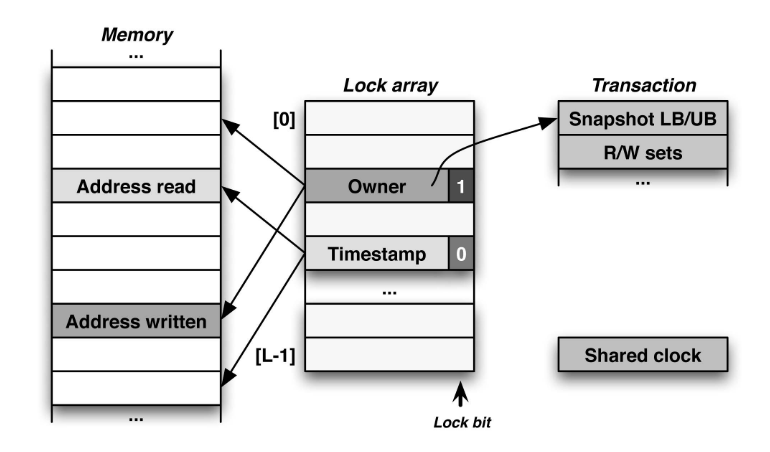
\includegraphics[width=\textwidth]{figures/background/TinySTMDataStructs.png}}
	\caption{Data structures utilized internally by the STM library \texttt{TinySTM}. Source: \cite{TinySTM2}. R/W sets stands for read and write sets. A snapshot corresponds to a range of valid linearization points. LB and UB stand for lower and upper bounds, i.e, the validity range of the snapshot.}
 	\label{fig:TinySTMDataStructs}
\end{figure} 

Figure \ref{fig:TinySTMDataStructs}, represents the internal organization of \texttt{TinySTM}. Each transaction has two internal linked lists, called read-set (RS) and write-set (WS). These lists are utilized to keep track of memory locations read and written by transactions. Another important data structure for STMs, is the lock array, implemented using a hash table. This table is utilized to map memory locations to their related versioned locks. When a versioned lock is locked, its last bit is set to one and the remaining bits contain the owner of the memory location. If the lock is free, it contains the current version of the memory location, also called timestamp (Figure \ref{fig:TinySTMDataStructs}). Some authors call the lock array as \emph{ownership records} (orecs), because it associates memory locations with their current owners \cite{NOrec}.

To summarize, a transaction performs the follow operations. To make it simpler, we do not intent to cover all possible algorithm cases. The main idea is to show the basics of how an STM algorithm works.

\begin{itemize}
	\item \textbf{Begin Transaction}: The current global clock value is copied to a local variable of the transaction. Normally, the variable name is $rv$ which stands for \textit{\textbf{r}ead \textbf{v}ersion}. This value will be utilized to validate reads on memory locations.
	
	%---------------------------------------------------------%
	\item \textbf{Read} or \textbf{Load}: 	With \textbf{eager} version management (Section \ref{sec:versionManag}), the transaction verifies if it owns the lock of the memory location that is being read. If true, it returns directly the value stored in memory. If the lock of the memory location belongs to another transaction, an abort is necessary.  Using \textbf{lazy} version management, the transaction first verifies if the memory location that it wants to read is in their WS. In that case, the transaction has already written to this location and the value in the WS must be returned. 
Otherwise, it is verified if the memory location is locked by another transaction. If true, an abort is necessary. Otherwise, the version associated with the memory location is compared with $rv$. If the version of the memory locations is greater than $rv$, an abort is necessary, as the memory location was updated after the transaction that is accessing it started. In case of abort, independently of the version management, the CM (Section \ref{sec:contetionManager}) is triggered. STM implementations, such as \texttt{TinySTM}, try to do additional processing before aborting a transaction, for instance, the use of \textit{timestamp extension} technique \cite{Riegel:2006}.
Finally, the address read is added to the RS and the content of the memory location is returned.
	
	%---------------------------------------------------------%
	\item \textbf{Write} or \textbf{Store}: 
First, it is necessary to verify if the memory location is locked. If true an abort is necessary.
The next step, in case of \textbf{eager} conflict detection (Section \ref{sec:conflictDetection}) is to lock the memory location.
If \textbf{eager} version management (Section \ref{sec:versionManag}) is utilized, the new value is updated directly on memory and the old one is stored in an undo-log. If the version management is \textbf{lazy}, the new value is stored in the WS to be updated at commit time.
	
	%	Conflict detection:
	%		Eager: locks is acquired now (tinystm)
	%		Lazy: lock is acquired only at commit-time (TL2)
	%	Eager version management:
	%		Update new value in memory and keep the old in a undo-log.
	
	%---------------------------------------------------------%
	\item \textbf{Commit}: 
Read-only transactions can commit directly, as the memory locations were validated on the \textbf{Read} step.
 For write transactions, the first step is to validate the RS, verifying each address, if it is locked by other transaction and if the $rv$ is still valid.
If the implementation uses \textbf{lazy} version management (Section \ref{sec:versionManag}), all address in the WS should be locked. If it fails, the transaction aborts. In case of eager version management, addresses have already been locked in the \textbf{Write} step.
Then, the global clock is advanced by 1 and the result is used as the new version for the values being updated. If \textbf{lazy} version management is used, the new values are updated in the memory. In the case of \textbf{eager} version management, the new values were updated in the \textbf{Write} step.
A final step, for both version managements, is to release the locks and set the new version value of the memory location.
	
	%	Lazy conflict detection: locks in the WS are acquired now. Fail to acquire then abort.
	
	%	Write transactions:
	%		Revalidate RS. If locked or rv < version number then abort.
	%		Advance global clock by 1
	%			If lazy version management: update new values in memory, release the lock and set new version value.
	%			If eager version management: ?
	%		Release locks 
	
	%------%
	%	Read-only transactions: Do not need increment the global clock, because no values are written to the memory.
	
	%---------------------------------------------------------%
	\item \textbf{Abort}: If the implementation uses eager version management, all values from the \emph{undo-log} must be restored. Otherwise, the \emph{redo-log} is discarded. 
A final step is to release all locks, if acquired.
\end{itemize}

%%%%%%%%%%%%%%%%%%%%%%%%%%%%%%%%%%%%
\section{Benchmarks for STM}\label{sec:STAMP}
%Synthetic and their own implementations
% linked list, integer set, bank
%sets and lists and trees.
Together with the first STM proposals, researches also developed benchmarks for testing. In most of the cases, these benchmarks were simple, based on sets, lists and maps \cite{Herlihy:2003_2, Harris:2003, Scherer:2005, Riegel:2006, Dice:2007}. Hence, it was necessary to develop specific TM benchmarks to evaluate TM systems. More specifically, benchmarks with realistic characteristics. One of the first benchmarks proposed for evaluating STM systems were \texttt{STMBench7}~\cite{STMBench7} and \texttt{Lee-TM}~\cite{LeeTM}. After that, other suites and standalone benchmarks applications were proposed to evaluate TM systems, for instance, \texttt{Eigenbench}~\cite{Eigenbench}, \texttt{RMS-TM}~\cite{Kestor:2011}
and, \texttt{Memcached}~\cite{Ruan:2014_2}.

Despite the effort on STM benchmarks proposal, the most used for evaluating TM implementations is the \texttt{STAMP} (\textit{Stanford Transactional Applications for Multi-Processing})~\cite{STAMP}. This suite is composed of 8 applications with realistic characteristics and that represent several application domains. \tablename~\ref{tab:stampSummary} shows the domain and a short description of each application from \texttt{STAMP} benchmark.

\begin{table}[!tb]
	\centering
	\caption{Applications from \texttt{STAMP} benchmark. Source: \cite{STAMP}.}
	\label{tab:stampSummary}
	\begin{tabular}{@{}lll@{}}
		\toprule
		\textbf{Application} & \textbf{Domain}               & \textbf{Description}                   \\ \midrule
		bayes                & machine learning              & Learns structure of a Bayesian network \\
		genome               & bioinformatics                & Performs gene sequencing               \\
		intruder             & security                      & Detects network intrusions             \\
		kmeans               & data mining                   & Implements K-means clustering          \\
		labyrinth            & engineering                   & Routes paths in a maze                   \\
		ssca2                & scientific                    & Creates efficient graph representation \\
		vacation             & online transaction processing & Emulates travel reservation system     \\
		yada                 & scientific                    & Refines a Delaunay mesh                \\ \bottomrule
	\end{tabular}
\end{table}

%The \texttt{STAMP} benchmark suite is composed of these applications:

%\begin{itemize}
%	\item \textbf{bayes}: 
%	\item \textbf{genome}: 
%	\item \textbf{kmeans}: 
%	\item \textbf{labyrinth}: 
%	\item \textbf{ssca2}: 
%	\item \textbf{vacation}:
%	\item \textbf{yada}:
%\end{itemize}


\texttt{STAMP} still is the most used STM benchmark suite, as can be seen in recent researches~\cite{Chen:2020, Carvalho:2020, Sanzo:2020, Yu:2019, Poudel:2019, Mururu:2019}.


%%%%%%%%%%%%%%%%%%%%%%%%%%%%%%%%%%%%
\section{Sharing-Aware Mapping}\label{sect:sharing-aware}

Data locality is an important factor in modern multicore and NUMA systems. One way to better explore locality is to map threads and data according to their \emph{memory access behavior} \cite{Diener:2016Sur}. Hence, two types of mappings are possible \cite{Cruz:2018}:
\begin{enumerate}
	 \item \textbf{Thread mapping}: threads are associated to cores, improving the cache usage and interconnections, i.e., threads are mapped to cores that are close to each other in the underlying architecture.

	\item \textbf{Data mapping}: memory pages are associated with NUMA nodes, optimizing the usage of memory controllers, i.e., memory pages are mapped to the same NUMA node where the core that is accessing them belongs.
\end{enumerate}

Thread and data mapping based on the memory access behavior of applications is called \textbf{sharing-aware mapping} \cite{Cruz:2018}. Although the Linux kernel handles thread and data mapping, for thread mapping it does not take memory access patterns into consideration. For instance, the \emph{Completely Fair Scheduler} (CFS) \cite{Wong:2008} used by default in the Linux kernel \cite{Diener:2016Sur} mainly focuses on load balancing. For data mapping, the default policy is called \emph{first-touch} \cite{Gaud:2015} where the memory is allocated in the NUMA node where the first access to the memory page is performed. Another data mapping policy available is \emph{interleave}, that focuses on balance, allocating pages in a round-robin way on the NUMA nodes \cite{Lameter:2013}.

To perform a thread mapping, it is necessary to know how threads share data \cite{Diener:2016Sur}. This information is usually represented as a \emph{communication matrix}~\cite{Bordage:2018}. Also required is information about the hardware hierarchy, which can be discovered using tools such as \texttt{hwloc}~\cite{hwloc}. A mapping algorithm uses the communication matrix and hardware hierarchy to choose an improved mapping of threads to cores.

For data mapping based on memory access, the accesses of each NUMA node to  pages must be known~\cite{Cruz:2018}. Current systems have millions or even billions of memory pages. For this reason, only a small group of pages must be considered for the mapping decision, avoiding a high overhead \cite{Diener:2016Sur}.

As mentioned in Section~\ref{sect:motivation}, STM provides interesting mapping opportunities since the STM runtime has precise information about memory areas that are shared between threads. The main idea of this thesis is to use information about transactional shared variables inside STM runtime to perform an efficient mapping. Hence, this thesis will focus on sharing-aware \textbf{thread mapping}. For efficient data mapping is necessary to have a global vision of the memory pages of an application, not only the ones accessed by the STM runtime. Nevertheless, in Appendix~\ref{chap:sharAwareDataMap} we made some experiments with sharing-aware data mapping in STM to confirm this hypothesis.

\subsection{Communication/sharing matrix}\label{sect:commMatrix}

To determine a better placement of threads and data, an affinity measure is required. For thread mapping, a common measure is a communication or sharing matrix~\cite{Bordage:2018, Mazaheri:2018}, in which each cell represents the amount of communication between pairs of threads~\cite{Sasongko:2019}. Since the amount of communication between thread $i$ and $j$ is the same between $j$ and $i$, the communication matrix is symmetric and diagonals are zero~\cite{Mazaheri:2018}. \figurename~\ref{fig:comMatrExample} shown examples of communication matrices, where axes show thread IDs. 
\begin{figure}[!ht]
	\centering
	\subfigure[Numbered matrix.]{
		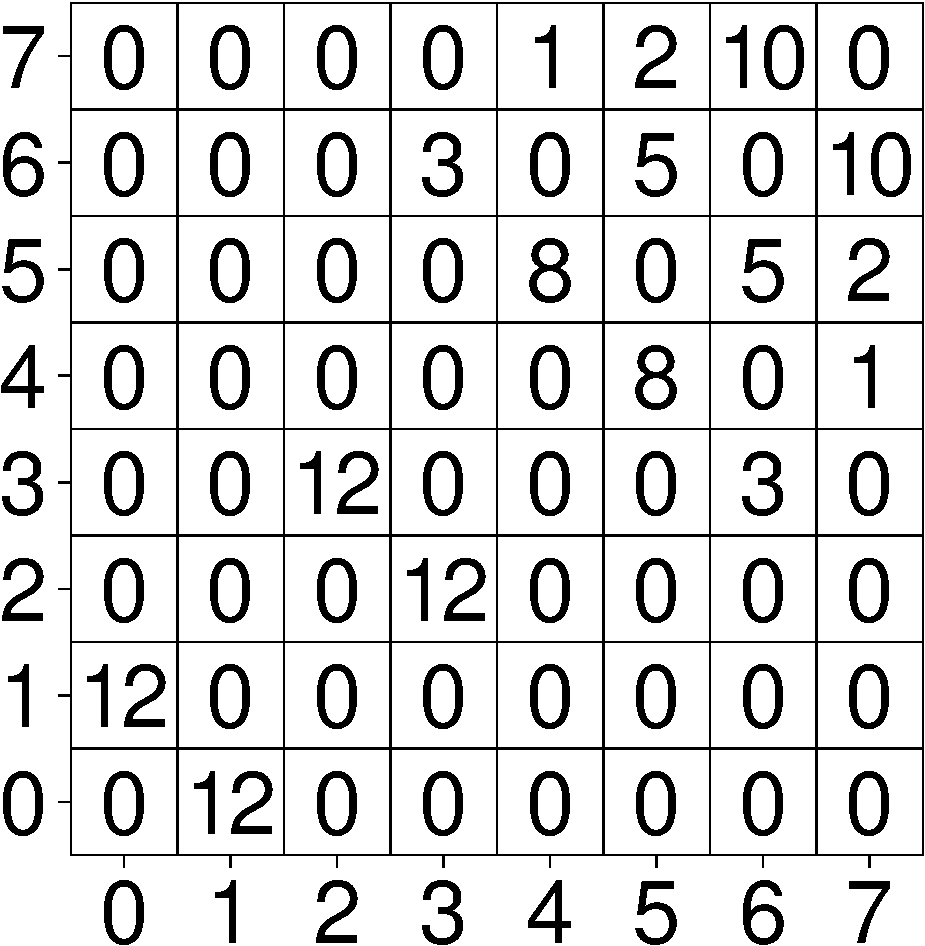
\includegraphics[width=0.3\textwidth]{figures/background/comm_matrix_num.pdf}
		\label{fig:comMatrNum}
	}
\hspace*{1cm}
	\subfigure[Colored matrix (heatmap).]{
		\label{fig:comMatrGraph}
		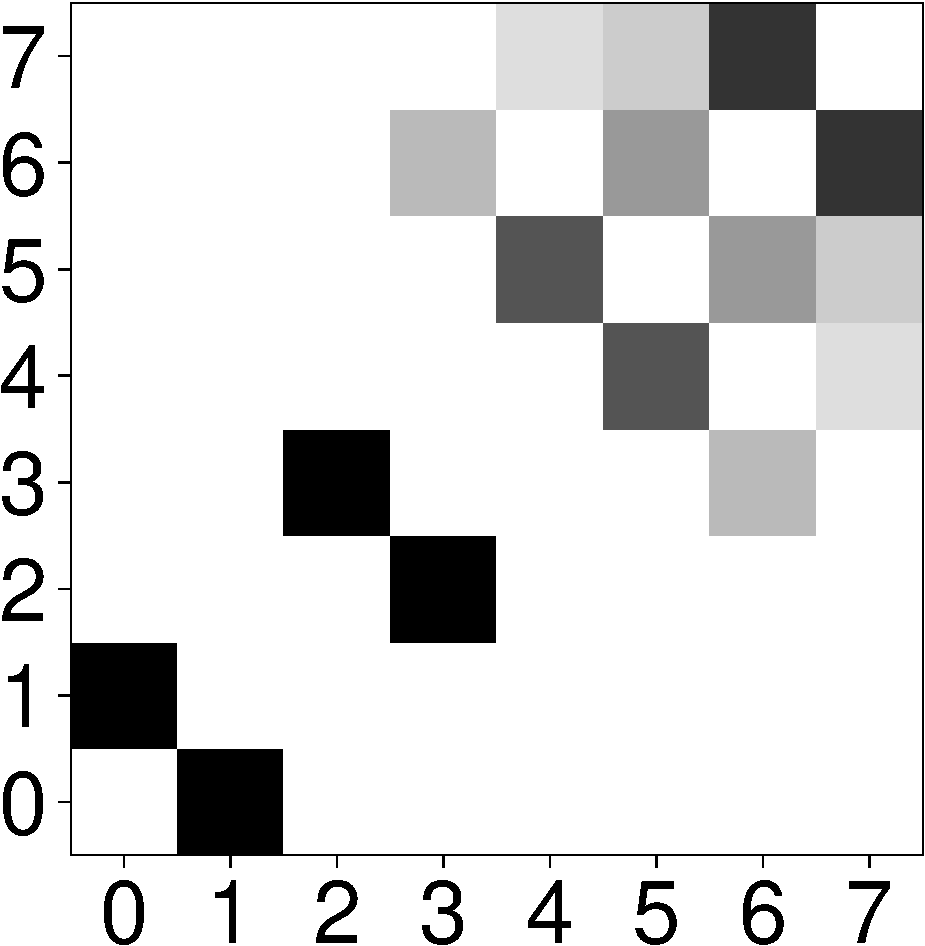
\includegraphics[width=0.3\textwidth]{figures/background/comm_matrix_graph.pdf}
	}
	\caption{Examples of communication matrices}
	\label{fig:comMatrExample}
\end{figure}
In \figurename~\ref{fig:comMatrGraph}, the matrix is represented graphically, where darker cells indicate more communication between pairs of threads~\cite{Diener:2016:2}.

\section{Improving STM applications with Thread Mapping}\label{sec:improvements}

To show how  sharing-aware thread mapping can improve the performance of an STM application, we designed an experiment that illustrates sharing-aware mapping of an STM application that calculates the sum of 16 million array elements. In the application, each group of 2 threads computes the sum of their respective array part in a shared sum variable. For example, with 8 threads, there are 4 shared variables for computing the sum.  The memory access behavior is known in advance: threads 0 and 1 access a shared variable, threads 2 and 3 another shared variable, and so on. Algorithm~\ref{alg:arraySumThread} shows how the sum function works. Lines \ref{alg:arraySumFirstLine}-\ref{alg:arraySumLastLine} verify the number
of the thread that is performing the sum and stores it in the respective shared variable. Thus, keeping threads that share a sum variable on sibling cores improves the cache usage. We used the \texttt{TinySTM}~\cite{TinySTM2} library for the synchronization of shared variables, with the default configuration: \emph{lazy} version management, \emph{eager} conflict detection and CM \emph{suicide}.

\begin{algorithm}[!tb]
	\caption{Function executed by each thread on the array sum application}\label{alg:arraySumThread}
	\small
	\begin{algorithmic}[1]
		\Function{sum}{}
		\Require
		\Statex \textbf{tid}: thread ID that is accessing this function
		\Statex
		\State \text{pinThreadToCore(tid, coreId)} \Comment{bind thread to core according to the strategy}
		\ForAll{value in array}
			\State	\text{stm\_start\_transaction()}   \Comment{begin transaction}
			\If{$(tid$ \text{in} $0,1)$}    \label{alg:arraySumFirstLine}
				\State \text{\textbf{stm\_write}(sum\_0\_1, \textbf{stm\_read}(sum\_0\_1) + \textbf{stm\_read}(value))}
			\ElsIf{$(tid$ \text{in} $2,3)$}
				\State \text{\textbf{stm\_write}(sum\_2\_3, \textbf{stm\_read}(sum\_2\_3) + \textbf{stm\_read}(value))}
			\ElsIf{$(tid$ \text{in} $4,5)$}
				\State \text{\textbf{stm\_write}(sum\_4\_5, \textbf{stm\_read}(sum\_4\_5) + \textbf{stm\_read}(value))}
			\ElsIf{$(tid$ \text{in} $6,7)$}
				\State \text{\textbf{stm\_write}(sum\_6\_7, \textbf{stm\_read}(sum\_6\_7) + \textbf{stm\_read}(value))} \label{alg:arraySumLastLine}
			\EndIf
			\State	\text{stm\_commit()}   \Comment{try to commit}
		\EndFor
		\EndFunction
	\end{algorithmic}
\end{algorithm}

We executed this application on the following NUMA machines: \textit{Xeon}, with 8 Intel E5-4650 processors, totaling 96 cores and 8 NUMA nodes and \textit{Opteron}, with 4 AMD Opteron 6276 processors, totaling 64 threads and also 8 NUMA nodes (more details on the machines in Section~\ref{sect:threadMapMethodology}). For the tests, 4 different configurations were used: the default ``Linux scheduler'', ``no cache sharing'', ``Cache sharing - Balance'' and ``Cache sharing - Socket''. With exception of ``Linux scheduler'', the mapping strategies are shown in \figurename~\ref{fig:MappingStrategyArraySum}.

\begin{figure}[ht]
	\centering
	\subfigure[No cache-sharing.]{
		\label{fig:MappingStrategyNoShare}
		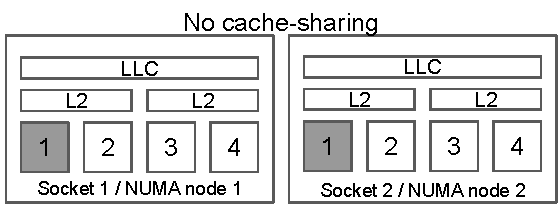
\includegraphics[width=0.48\textwidth,trim=0 0 0 17,clip]{figures/background/map-no-share.pdf}
	}%
	\subfigure[Cache sharing - Balance.]{
		\label{fig:MappingStrategyBalance}
		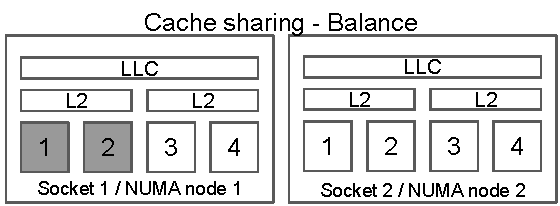
\includegraphics[width=0.48\textwidth,trim=0 0 0 17,clip]{figures/background/map-balance.pdf}
	}%
	\\
	\subfigure[Cache sharing - Socket.]{
		\label{fig:MappingStrategySocket}
		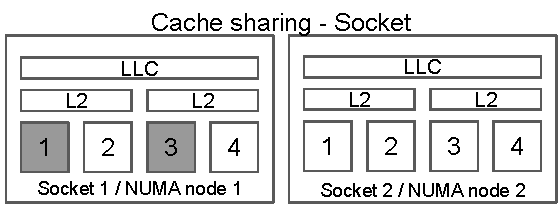
\includegraphics[width=0.48\textwidth,trim=0 0 0 17,clip]{figures/background/map-socket.pdf}
	}%
	\caption{Thread mapping strategies for the Array Sum application.}
	\label{fig:MappingStrategyArraySum}
\end{figure}

The idea of ``no cache sharing'' is to map threads that share the same variable to different NUMA nodes, forcing remote accesses and cache coherency messages between the nodes. In contrast, in the ``Cache sharing - Balance'' approach, the idea is to map threads that share a variable to sibling cores on the same NUMA node to share caches. However, for this configuration we map each pair of shared variables to different sockets.


Finally, for ``Cache sharing - Socket'', the idea is to place threads on sibling cores, sharing all cache levels. Since this application uses 8 threads, using this configuration all threads will be mapped to only one socket. To pin threads to cores the function \texttt{pthread\_setaffinity\_np} was utilized. The mapping was applied when a thread calls the function \texttt{stm\_init\_thread} of the \texttt{TinySTM} library. This function informs the STM runtime that the thread that has called it will perform transactional operations. \figurename~\ref{fig:arraySum} presents the execution time in seconds on each machine.


\begin{figure}[!ht]
	\centering
	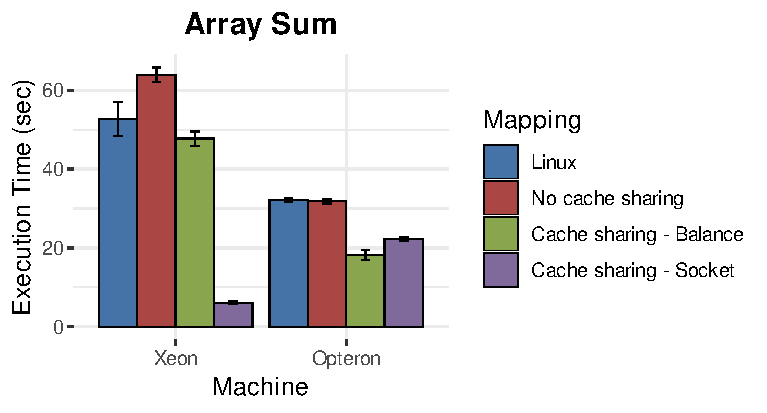
\includegraphics[width=0.7\textwidth]{figures/background/arraySum.pdf}
	\caption{Execution time of the Array Sum application.}
	\label{fig:arraySum}
\end{figure}


On the Opteron machine, the Linux scheduler had similar results as the ``no cache sharing''  configuration. When the application was running, we observed that the scheduler tries to balance threads, distributing them to the NUMA nodes, without taking the sharing behavior into account. This explains that the results are similar to ``no cache sharing''. On Xeon, the NUMA effects are more clear since forcing threads to run on distinct sockets, i.e., ``no cache sharing'' configuration, presented the worst performance.

%hurts the performance more than the Linux Scheduler.


For the ``Cache sharing - Balance'' configuration, on Xeon the execution time was reduced by 9.46\% whereas in Opteron it was reduced by 43.02\%. However, the most interesting result appears using ``Cache sharing - Socket'' mapping on the Xeon. Using this configuration, the execution time was reduced by 88.46\%. Although in Opteron the result of ``Socket'' was also positive (30.69\% of reduction time), the ``Balance'' configuration was better. We think that the good results of ``Socket'' on Xeon can be explained by the size of the last-level cache (LLC). The size of the data structures used by the array sum is 64MB. The size of LLC of the Xeon is 30MB whereas in Opteron it is 6MB. In that case, almost half of the memory used by the application fits entirely on the LLC of the Xeon. For the Opteron, mapping the variables to distinct cores increases the performance gains compared to ``Socket'' configuration, because more cache was available to the application.


\section{Summary}
This chapter presented the background related to this thesis. It also included a small experiment with a synthetic application to illustrate the possible benefits of sharing-aware thread mapping for STM applications.
